\subsection*{1. Diagrama del proceso}

A continuación se presenta el diagrama del proceso de recepción y control de calidad de la fruta, con las respectivas capacidades en cada etapa.

\begin{figure}[H]
    \centering
    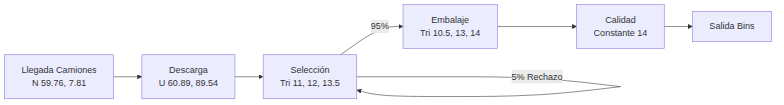
\includegraphics[width=0.9\textwidth]{p1/diagrama_p1.png}
    \caption{Diagrama de flujo del proceso.}
\end{figure}

\subsection*{2. Distribución de llegada}

El tiempo entre llegadas de los camiones se modela como una distribución Normal, y la descarga como una distribución Uniforme, de acuerdo con la validación de datos.

\subsection*{3. Resultados de simulación: utilización y tiempos}

\subsection*{4. Identificación del cuello de botella}

\subsection*{5. Multas por pérdida de calidad}

\subsection*{6. Ubicación del control de calidad}

\subsection*{7. Reducción de variabilidad (Selección vs Embalaje)}

\subsection*{8. Cambios en un mes de funcionamiento}
